\chapter{Simulation procedure}
% \todob{In experiments: mention smaug}
\todobo{In experiments: mention phase transitions of silica and water? Water has same phase even if we have high pressure/density}
\todobo{Steepest descent procedure?}
\section{Initialization\label{sec:experimental_procedure}}
When doing simulations using molecular dynamics we use a procedure akin that used by actual experiments. Since the duration of the simulations we are realistically able to simulate on are of the order of tens of nanoseconds, we have to be smart when initializing the system, to avoid having to simulate for a long time to get to the state we want to study. This means that we should start out with the system in a state as close to the one we want to study as possible. The problem with this when simulating silica is that the silica structure formed when rapidly cooling molten silica does not have any long-range ordering. Silica in the glass form has an amorph structure, which does not have any long-range ordering, but has short-range ordering well beyond the Si-O bond length. This structure is hard to set up with an algorithm.

To generate silica in the glass form we first create a perfect silica crystal in the crystalline form $\upbeta$-cristobalite, the unit cell of which can be seen in figure \cref{fig:beta_cristobalite-unit_cell}, and a larger crystal in \cref{fig:cristobalite_crystal}. This crystalline form consists of corner-bonded SiO$_4$-tetrahedra, and in the perfect crystallic form all silicon atoms are bound to four oxygen atoms, and all oxygen atoms to two silicon atoms. 

We give the atoms a random uniformly distributed velocities with mean $\mu = 0$ and standard deviation $\sigma \propto \sqrt{T}$, where $T$ is the wanted temperature.%
\begin{figure}[htb]%
    \centering%
    \includegraphics[width=0.4\textwidth]{images/beta_cristobalite/unit_cell05_cropped.png}%
    \caption{%
        $\upbeta$-cristobalite unit cell, with 8 silicon atoms and 16 oxygen atoms.%
        \label{fig:beta_cristobalite-unit_cell}%
    }%
\end{figure}%

We then heat the system to 4500 K in steps of 700 K to melt the silica crystal. Since we are mainly interested in controlling the temperature at this stage, the Berendsen thermostat is used for these temperature changes. We alternate between using a thermostat to adjust the temperature, and simulating with the thermostat off, to let the system thermalize and react to the temperature change after applying the thermostat. The number of timesteps we used for the thermostat period is around 2 500, and for the thermalization period around 10 000. We then cool the system by doing the previous procedure in reverse. See \cref{fig:plot_heat_melt_sio2} for a plot of the temperature as function of time while we melt and cool down the system, and \cref{fig:initialization_step00} for a visualization of a perfect crystal of $\upbeta$-cristobalite, and \cref{fig:initialization_step02} for amorphous, solid silica.%
%
\begin{figure}[htpb]%
    \centering%
    \includesvg[width=0.6\textwidth, svgpath = ./images/energy_plots/]{system00_temperature_melt_cool}%
    \caption{%
        Plot of the temperature (in kilo-Kelvin) as function of timesteps when melting and cooling down a silica system, using the Berendsen thermostat. We use timesteps of 0.050 picoseconds, and use 2 500 timesteps with the thermostat turned on, and then 10 000 timesteps to let the system thermalize (with the thermostat off), for each step in temperature. %
        \label{fig:plot_heat_melt_sio2}%
    }%
\end{figure}%
%
% \todob{Reference figures below, say something about energy conservation \cref{fig:plot_heat_melt_sio2,fig:plot_energy_conservation}}
% \todoco{Silica phase diagram? for melting, phases etc. - Not needed according to Malthe}

The initialization procedure is visualized in \cref{fig:initialization_steps}, and can be summed up as follows
\begin{itemize}
    \item Generate a perfect crystal of $\beta$-cristobalite of the wanted size (\cref{fig:initialization_step00}).
    \item Heat the system to well above the melting point of silica (we usually use 4 500 Kelvin, using a thermostat (Berendsen) (\cref{fig:initialization_step01}).
    \item Cool down the system to well below the glass-transition temperature (we use 300 Kelvin), using a thermostat (Berendsen) (\cref{fig:initialization_step02}).
    \item Cut out the fracture (\cref{fig:initialization_step03}).
    \item Passivate the dangling ends and apply steepest descent to let the passivation atoms find their optimal positions (\cref{fig:initialization_step04}).
    \item Fill the pore with water, and thermalize the system at 300 K (\cref{fig:initialization_step05}).
\end{itemize}
%
\begin{figure}[htpb]%
%     \captionsetup{width=1.4\textwidth}%
    \setlength{\myfigwidth}{0.35\textwidth}%
    %
    \setlength{\myhfillwidth}{1.5cm}%
    \centering%
    \begin{subfigure}[t]{\myfigwidth}
        \captionsetup{width=1.1\textwidth}%
        \includegraphics[width=\textwidth]{images/experimental_procedure/00_10}%
        \caption{%
            Perfect $\upbeta$-cristobalite crystal.%
            \label{fig:initialization_step00}%
            \label{fig:cristobalite_crystal}%
        }%
        \hspace{8pt}
    \end{subfigure}%
    \hspace{\myhfillwidth}%
    \begin{subfigure}[t]{\myfigwidth}%
        \includegraphics[width=\textwidth]{images/experimental_procedure/01_10}%
        \caption{%
            Silica heated to 4500 K.%
            \label{fig:initialization_step01}%
        }%
        \hspace{8pt}
    \end{subfigure}%
    \\%
    \begin{subfigure}[t]{\myfigwidth}%
        \includegraphics[width=\textwidth]{images/experimental_procedure/02_10}%
        \caption{%
            Silica cooled to 300 K.%
            \label{fig:initialization_step02}%
        }%
    \end{subfigure}%
    \hspace{\myhfillwidth}%
    \begin{subfigure}[t]{\myfigwidth}%
        \includegraphics[width=\textwidth]{images/experimental_procedure/03_10}%
        \caption{%
            Fracture cut out.%
            \label{fig:initialization_step03}%
        }%
        \hspace{8pt}
    \end{subfigure}%
    \\%
    \begin{subfigure}[t]{\myfigwidth}%
        \includegraphics[width=\textwidth]{images/experimental_procedure/04_10}%
        \caption{%
            Dangling ends passivated.%
            \label{fig:initialization_step04}%
        }%
        \hspace{8pt}
    \end{subfigure}%
    \hspace{\myhfillwidth}%
    \begin{subfigure}[t]{\myfigwidth}%
        \includegraphics[width=\textwidth]{images/experimental_procedure/05_10}%
        \caption{%
            Pore filled with water.%
            \label{fig:initialization_step05}%
        }%
        \hspace{8pt}
    \end{subfigure}%
    \captionsetup{width=\textwidth}%
    \caption{%
        Visualizations of the different stages of initialization of a fracture in silica filled with water. We show a $75\times 75\times 25$ \AA\ slice of a much larger system $(172 \text{ \AA})^3$. The silicon atoms are yellow, the silica-oxygen blue, and hydrogen and water-oxygen red. %
        \label{fig:initialization_steps}%
    }%
\end{figure}%

We now have a thermalized and (hopefully) realistic silica crystal at near room temperature. From this crystal we cut out the fracture, passivate using one of the passivation methods, and fill the fracture with water molecules, \hl{and use steepest descent}. After filling the fracture with water we need to thermalize the system again, since the energy (and thereby the temperature) changes when we remove and insert atoms.

\section{Passivation}
In most silicates the silicon atoms have tetrahedral coordination, with four oxygen atoms surronding each silicon atom. When we remove silica- and oxygen-atoms to create a fracture, we do not take this into consideration. This means that we get dangling unsaturated bonds in the system, located near the surface of the pore. To rectify this we use a method called passivation, where we saturate and passivate the dangling bonds by inserting new atoms. 

\subsection{Water chemistry}
Since we are going to inject water into the pore later on, we want to use the constituents of water to passivate the system. We know that water autodissociates into H$^{+}$ and OH$^{-}$ via the following reaction
\begin{align*}
    \text{H}_2\text{O} \rightleftharpoons \text{H}^{+} + \text{OH}^{-},
\end{align*}
meaning that hydrogen (H) and hydroxide (OH) will be freely available in the system after filling the pore with water. On this background we choose to passivate the system using hydrogen and hydroxide. To avoid getting an acidic or alkaline system after the passivation procedure we should make sure to use equal parts hydrogen and hydroxide when passivating.

\subsection{Passivating using hydrogen and hydroxide}
After thermalizing our silica system we end up with a system consisting almost exclusively of SiO$_2$ tetrahedra. These tetrahedra are each formed by four oxygen atoms, one in each corner, and a silicon atom in the center. Each of these tetrahedra are then bonded to four other tetrahedra, by sharing the oxygen atoms in the corners. This way each oxygen atom is bonded to two silicon atoms, and each silicon atom to four oxygen atoms, giving an average chemical formula of SiO$_2$. 

Since we do not take chemical bonds into consideration when removing atoms to create a fracture, we end up with some incomplete tetrahedra, with some silicon atoms bonded to less than four oxygen atoms, and some oxygen atoms bonded to less than two silicon atoms. See \cref{fig:passivation} for an illustration of three different incomplete tetrahedra. This creates what we call dangling ends or unsaturated bonds, which we want to passivate.

% When inserting hydrogen and hydroxide we want to insert them in positions that are close to their equilibrium positions, so we do not have to do a lot of simulating to get a stabilized system after passivating. It is possible to calculate the optimal positions based on the potential and the positions of the existing atoms, but this is a complicated computation, that we can avoid, by instead realizing that the optimal positions for the oxygen atoms we insert will most likely \hl{(source?)} be close to the positions that complete the SiO$_2$ tetrahedra. These positions can be calculated, using simple geometry, from the positions of the oxygen atoms each silicon atom is bonded to.

To passivate the silicon atoms that are bonded to less than four oxygen atoms, we see that we need to complete the incomplete SiO$_4$ tetrahedra that have been created in the system. But if we only insert oxygen atoms in the positions of the missing oxygen atoms, we end up with new dangling ends, since the inserted oxygen atoms will only be bonded to one silicon atom. But, as we just saw, we will have hydroxide (OH) groups available in the system after filling the fracture with water. So instead of inserting oxygen atoms and creating new unsaturated bonds, we insert hydroxide groups and create saturated Si-O-H bonds. We put the hydrogen atom so that the Si-O-H angle is close to the angle in water molecules, 107.5 degrees. \hl{The hydrogen atoms moves very rapidly compared to the rest of the species in the system, so they will quicly find the equilibrium position, meaning that the exact position of the hydrogen atoms is not that important.}

To passivate the oxygen atoms that are bonded to only one silicon atom, we can use the hydrogen atoms that are avilable after filling the fracture with water, turning unsaturated SiO-groups into the same saturated Si-O-H-groups as before. We here too insert the hydrogen atoms with the Si-O-H angle close to 107.5 degrees.

In total we use the following procedure to passivate a system after creating a fracture:
\begin{itemize}
    \item Remove all silicon and oxygen atoms that are not bonded to any atoms, since they are essentially not part of the silica matrix.
    \item Add one hydrogen atom to all oxygen atoms bonded to only one silicon atom. The hydrogen atoms are inserted approximately $0.95\text{ \AA}$ from the oxygen atoms, with the hydrogen atom pointing away from the silicon atom, and with the Si-O-H angle close to 107.5 degrees.
    \item Add ($4-n$) hydroxide groups to silicon atoms bonded to $(1\leq n<4)$ oxygen atoms. We assume that the most stable position for the oxygen in the hydroxide groups are close to the tetrahedral positions of the missing oxygen atoms, and insert the hydroxide groups in these positions. %
    %See \cref{fig:pass_tet01,fig:pass_tet02,fig:pass_tet03} for the three different cases. 
    The hydroxide groups are inserted approximately $1.65\text{ \AA}$ from the silicon atoms, measured from the position of the silicon atom to the oxygen atom in the hydroxide groups, with the hydrogen atom pointing away from the silicon atom, and with the Si-O-H angle close to 107.5 degrees.
\end{itemize}
The lengths used are approximate experimental lengths found in naturally occuring silanols and water (see \cite{lickiss1995synthesis} for the Si-O length in silanol, and \cite{csaszar2005equilibrium} for the O-H length in water). This procedure turns all dangling ends into stable, passive silanol groups.
%
\begin{figure}[htpb]%
    \centering%
    \setlength{\myfigwidth}{0.17\textwidth}
    \begin{subfigure}[c]{0.8\myfigwidth}%
        \includegraphics[width=\textwidth]{images/passivation/tetrahedra01_01.png}%
        \caption{}%
%         \caption{Illustration of how to divide a convex hexahedron into five tetraheda.}%
        \label{fig:pass_tet01}%
    \end{subfigure}%
    \hspace{1cm}%
    \begin{subfigure}[c]{\myfigwidth}%
        \includegraphics[width=\textwidth]{images/passivation/tetrahedra02_01.png}%
        \caption{}%
%         \caption{A random fracture made from two periodic heightmaps.}%
        \label{fig:pass_tet02}%
    \end{subfigure}%
    \hspace{1cm}%
    \begin{subfigure}[c]{1.1\myfigwidth}%
        \includegraphics[width=\textwidth]{images/passivation/tetrahedra03_01.png}%
        \caption{}%
%         \caption{A random fracture made from two periodic heightmaps.}%
        \label{fig:pass_tet03}%
    \end{subfigure}%
    \hspace{1cm}%
    \begin{subfigure}[c]{1.1\myfigwidth}%
        \includegraphics[width=\textwidth]{images/passivation/tetrahedra04_01.png}%
        \caption{}%
%         \caption{A random fracture made from two periodic heightmaps.}%
%         \label{fig:fracture_model}\caption{}%
    \end{subfigure}%
    \caption{%
        Illustration of four different incomplete silica tetrahedra, with respectively one, two, three and no missing oxygen atoms (\textbf{(d)} is a complete silica tetrahedra).%
    }%
    \label{fig:passivation}%
\end{figure}%

\subsection{Counting number of bonds}
Since we do not have actual bonds in molecular dynamics simulations, we do not know which atoms are bonded to which. So to find the number of bonded atoms for each silicon and oxygen atom, we create what we call \emph{neigbor lists}. These neighbor lists are a list of atoms within a chosen radius for each atom. To create these lists we use the procedure detailed in \cref{sec:neighbor_lists}. Since we only have silicon and oxygen atoms in our system, we only need to specify a maximum the Si-O-distance to find which atoms are bonded. If we choose this distance properly, we should be able find a good approximation to how many atoms each atom is bonded to.
\todobo{Something about g(r) for deciding Si-O bond length, or potential parameters?}

\orangebox{
\begin{itemize}
    \item What Si-O distance did we use to find bonds? Why? 
    \item g(r) for Si-O?
    \item Implementation?
    \item Visualization of results?
    \item What to do about atoms that can not be passivated (because we have to insert passively)?
\end{itemize}
}

% \subsection{Implementation}
% To implement the passivation procedure detailed above we see that we can make an  

% \begin{itemize}
%     \item Tetrahedra
%     \item Neighbor lists -- see base\_code/passivate\_using\_tetrahedra/passivator.cpp near line 700
%     \begin{itemize}
%         \item Create list of atoms in each voxel
%         \item Create neighbor lists for each atom by looping through neighbor voxels for each atoms
%     \end{itemize}
%     \item Count number of neighbors of different types -- find number of missing neighbors, Si - 4 Oxygen, Oxygen 2 Si
%     \item Insert OH on Si with missing O neighbors, insert H on Oxygen with missing Si neighbors
%     \begin{itemize}
%         \item Insert O/H at good angles
%     \end{itemize}
%     \item Improvement: find the atoms near surface using voxels, only passivate those atoms
% \end{itemize}

\subsection{Only passivating surface atoms}
When implementing the passivation method detailed above, we soon ran into problems with silica and oxygen atoms that were bonded to too few atoms according to our rules above, while counting the number of bonds using a fixed radius. Some improvements were made by fine-tuning the radius used for each atom type, but we still often ended up passivating atoms that were inside the silica matrix, where we should not have any dangling bonds. To avoid this we came up with a method to only passivate the atoms at or near the surface of the fracture.

To do this we yet again use the voxelation method from \ref{sec:voxelation}, but this time we use a voxel size of around $6\text{ \AA}$. We then mark all voxels with atoms in them as occupied. We now see that if we find all \emph{occupied} voxels with at least one \emph{unoccupied} neighbor voxel (using 26-neighbor connectivity), we should have a list of the voxels that make up the surface of the fracture, and these voxels then contain all atoms at or near the surface of the fracture. We then use this list of atoms as input to the passivation program, and only passivate atoms in that list. See \cref{fig:find_surface_atoms} for an illustration of the method that finds the voxels and atoms at the surface of the fracture.
%
\begin{figure}[htpb]%
    \centering%
    \includesvg[width=0.5\textwidth, svgpath = ./images/passivation/]{select_surface_voxels06}%
    \caption{%
        Illustration of a method for finding atoms and voxels at the surface of a fracture. All gray voxels are occupied voxels (with at least one atom in them), and the dark gray voxels are the voxels with at least one unoccupied neighbor voxel. %
        %\hl{FINISH} \hl{change to v1 of illustration?} \hl{what size shoud fig be? 0.4 maybe a bit small?}%
    }%
    \label{fig:find_surface_atoms}%
\end{figure}%

\subsection{Passivation examples}
An example of a system after passivation can be seen in \cref{fig:passivation_example}, where we have colored the passivating oxygen and hydrogen atoms red.
%
\begin{figure}[htpb]%
    \centering%
    \includegraphics[width=0.7\textwidth]{images/passivation/passivation_example04.png}%
    \caption{
        Example of the result of the passivation procedure. Here the oxygen and hydrogen molecules are red, silicon atoms are yellow, and silicon-oxygen atoms are light yellow.%
    }%
    \label{fig:passivation_example}%
\end{figure}%

\todobo{Decide on whether to include silanol density stuff, and if so, write it}
\orangebox{
A good measure of the performance of the passivation method is the surface density of silanol after passivation. This number is often called the \emph{silanol number}, and us considered to be a physico-chemical constant, with a numerical value $\alpha_\text{OH} = 4.6$ (least-squares method) and $\alpha_\text{OH}\text{ nm}^{-2}$ (arithmical mean) \cite{zhuravlev1999silanol}, and is known in literature as the Kiselev-Zhuravlev constant. As we will see, measuring the surface area of porous system is not trivial, so estimating this density is not trivial. But by creating a completely flat pore and passivating it, we found that we created a silanol surface density of $\approx 7.05\text{ nm}^{-2}$ (if counting number of inserted hydrogen atoms) or $\approx 3.53\text{ nm}^{-2}$ (if counting number if inserted oxygen atoms). MAYBE MEASURE THIS PROPERLY?

If the big number (7): since we inserted neutrally, the excess atoms will diffuse into the water anyway
If the small number: the water we inject later will passivate the rest of the atoms
Could also be caused by how we cut??
The surface area is really bigger than $L^2$, since the atoms make a ``rough'' surface, not flat.
}


\FloatBarrier
\section{Injecting water}
After removing atoms to create a fracture, and passivating the system, we are now ready to inject water into the fracture. To do this we use the technique of \emph{voxelation} (see \cref{sec:voxelation}). We first divide the system into voxels, find the voxels that make up the void, and then put water molecules in these voxels. The water density can then be controlled by the size of the voxels we use, and how many of the voxels we fill.

% \orangebox{
% \begin{itemize}
%     \item This could/should have been done using grand canonical ensemble / grand canonical monte carlo -- but this is computationally heavy?
%     \item The voxelation technique has problems in thin and/or skewed pores (not horizontal/vertical)
%     \item We want to have a water phase that is realistic (can be realistic with low or high density and pressure) and liquid
% \end{itemize}
% }

\subsection{Finding correct voxel size}
If we want to inject water with density $\rho$% [kg/m$^3$]
, we can find the voxel size we need from the molar mass of water, $M_\text{H$_2$O} = M = 0.0180158 \text{ kg/mol}$\todobo{source?}. We use the molar mass and wanted density to find the ``volume'' each water atom should occupy% , the unit used in the \hl{MD integrator/program and output files}
, as follows
\begin{align*}
    V 
    = \frac{ M\text{ [kg/mol]} \times \dfrac{1}{N_A \text{ [mol$^{-1}$]}}}{ \rho\text{ [kg/m$^3$]} } 
    = \frac{M}{\rho N_A}\text{[m$^3$]}
\end{align*}
where $N_A$ is the Avogadro constant. From here we find the size of the voxels by taking the cube root
\begin{align}
    l = \left(\frac{M}{\rho N_A} \right)^{1/3}\text{ m}.
    \label{eq:inject_water_voxel_size}
\end{align}
To get a water density approximately equal to $\rho$ we can then use a voxel size $l$, and put one water atom in each voxel. If we for example want to insert water with $\rho = 1000\text{ kg/m}^3$, approximately the density of water in room temperature\todobo{source?}, we get a voxel size of
\begin{align*}
    l = \left(\frac{0.0180158 \text{ kg/mol}}{1000\text{ kg/m$^3$} \times 6.0221 \times 10^{23}\text{ mol$^{-1}$}} \right)^{1/3} = 3.1 \text{ \AA}.
\end{align*}

\subsubsection{Voxel size in finite systems}
Since we have a finite system we usually ca not use the exact voxel size we want, but we have to divide the system into an integer number of voxels. This means that we will not get the exact density we want if we fill all voxels. To remedy this we only fill the fraction of voxels to get the wanted density.

In practice we use the following procedure
\begin{itemize}
    \item Find the number of voxels to divide the system into (in each direction) via
    \begin{align*}
        n_i = \left\lceil \frac{L_i}{l_i} \right\rceil,
    \end{align*}
    where $L_i$ is the system size in dimension $i$ and $l_i$ is the voxel size calculated using \cref{eq:inject_water_voxel_size}. We use the ceiling-function to ensure that the actual voxel size we use is smaller than (or equal to) the voxel size we calculated. We find the actual voxel size via
    \begin{align*}
        \tilde l_i = \frac{L_i}{n_i}.
    \end{align*}
%     \item Mark all voxels within \hl{what radii?} as occupied.
    \item Divide the system into voxels of size $(\tilde l_x, \tilde l_y, \tilde l_z)$, and find the voxels that make up the void (see \cref{sec:inject_water_find_empty_voxels} for more on this).
    \item To find the ratio of voxels to put water molecules in we first calculate the density we would get if we filled all empty voxels using
    \begin{align*}
        \tilde\rho = \frac{M}{\tilde l_x \tilde l_y \tilde l_z N_A},
    \end{align*}
    and then find the number of voxels to fill as
    \begin{align*}
        \tilde N = N\frac{\tilde\rho}{\rho} = N\frac{\tilde l_x \tilde l_y \tilde l_z}{l_x l_y l_z},
    \end{align*}
    where $N$ is the total number of empty voxels.
    %\item \hl{Put a water molecule $\tilde N$ voxels}. 
    
    This can for example be done by looping over all voxels, drawing a random uniform number between 0 and 1 for each voxel, and putting a molecule in the voxel if the random number is smaller than $\tilde N / N$.
%     \begin{listing}[!htb]%
%         \begin{cppcode*}{gobble=12}
%             for (int i = 0; i < voxels.size(); i++)
%             {
%                 if (rand() < n_voxels_to_fill/n_voxels)
%                 {
%                     voxels[i].push_back(create_random_water_atom());
%                 }
%             }
%         \end{cppcode*}
%     \caption{%
%         \hl{FINISH THIS LISTING}.%
% %         \label{list:sampling}%
%     }%
%     \end{listing}%
\end{itemize}
The water molecules are inserted with the oxygen atom in the center of the voxel, and the two hydrogen atoms pointing in a random direction, but with an angle of $\sim 104.45^\circ$.

% \subsection[Finding empty/unoccupied voxels]{Finding \hl{empty/unoccupied} voxels\label{sec:inject_water_find_empty_voxels}}
\subsection{Identifying the voxels that make up the void\label{sec:inject_water_find_empty_voxels}}
The naive way of finding the voxels to fill with water is to just find which voxel each silicon and oxygen atom is in, and mark those as occupied. Using this method we found that we often got some empty voxels inside the silica matrix, which meant we got single water atoms trapped inside what was supposed to be the silica matrix. 

This can be explained if we compare the voxel size of $3.1 \text{ \AA}$ in water with a density of $\rho = 1000\text{ kg/m$^3$}$, as we found above, to the typical bond length between silica tetrahedra in solid silica, which is about \hl{???}. When we take into account the amorphous structure of silica we see that it is likely that we get some small pores with room for a water atom in between some of the silica tetrahedra.\todoao{better explanation}

To solve this we assign a radius to each atom type, and mark all voxels with the center of the voxel within this radius from an atom as occupied. The rest of the voxels should now be a good approximation to the void. See \cref{fig:inject_empty_voxel} for an illustration of this procedure. 
%
\begin{figure}[htpb]%
    \centering%
    \begin{subfigure}[b]{0.45\textwidth}%
        \includesvg[width=\textwidth, svgpath=./images/inject_water/]{drawing02}%
%         \caption{}%
        \caption{Marking only one voxel per atom as occupied.}%
%         \label{fig:pass_tet01}%
    \end{subfigure}%
    \hspace{0.05\textwidth}%
    \begin{subfigure}[b]{0.45\textwidth}%
        \includesvg[width=\textwidth, svgpath=./images/inject_water/]{drawing_radius02}%
%         \caption{}%
        \caption{Marking all voxels within radius from atom as occupied.}%
%         \label{fig:pass_tet02}%
    \end{subfigure}%
    \caption[
        To find voxels that make up the void/pore in we can either \textbf{a)} mark the voxel each existing atom belongs in as occupied, or \textbf{b)} mark all voxels within a radius from each atom as occupied. We can assign a different radius to each atom. We have illustrated using part of a silica tetrahedra, with one silicon atom (the large blue dot) and two oxygen atoms (the smaller red dot). The center of each voxel is marked by a dot 
    ]{%
        To find voxels that make up the void/pore in we can either \textbf{a)} mark the voxel each existing atom belongs in as occupied, or \textbf{b)} mark all voxels within a radius from each atom as occupied. We can assign a different radius to each atom. We have illustrated using part of a silica tetrahedra, with one silicon atom (\includegraphics[scale=0.8]{./images/inject_water/silicon.pdf}) and two oxygen atoms (\raisebox{0.3ex}{\includegraphics[scale=0.8]{./images/inject_water/oxygen.pdf}}). The center of each voxel is marked by a dot. %
        %\hl{Maybe change to v01 of images?} \hl{This voxel size is pretty tiny...}%
    }%
    \label{fig:inject_empty_voxel}%
\end{figure}%

\hl{A different solution to the problem of tiny pores inside the silica matrix is to remove all small clusters of voxels (where a ``small cluster of voxels'' would need to be defined), or maybe to use different voxel sizes for finding the void and filling the void with water.}\todoao{Fix or remove}

% \orangebox{
% \begin{itemize}
%     \item Remove tiny pores?
%     \item Give voxels random velocity based on wanted temperature? Now using zero!
%     \item Mark all voxels within distance from other atoms as occupied
%     \item Fill other voxels with H2O with random O-H orientation, but correct angle
%     \item Improvement: Use one voxel size in the beginning (to avoid one-voxel pores), and then use a smaller voxel size when injecting water
% \end{itemize}
% }

